\label{sec:appendix}
\section{Appendix}
% Modelling elevator motion
\subsection{Boltzmann Instability}

We select actions by computing the Boltzmann distribution over $Q$-values in a state. However, computing
\[
\frac{e^{Q_1/T}}{e^{Q_1/T} + e^{Q_2 / T}}
\]
is numerically unstable. The fraction will be imprecise, since the value of both the denominator and numerator will be extremely large. At a certain point it becomes impossible to even calculate the exponentials. We use a little trick to remedy this. Let $Q_* = \max(Q_1/T, Q_2/T)$. Then we compute
\[
\frac{e^{Q_1/T - Q_*}}{e^{Q_1/T - Q_*} + e^{Q_2 / T - Q_*}}
\]
which is mathematically equivalent to the above but numerically stable.

\label{sec:solving_integral}
\subsection{Solving Return Integral}

To compute returns, we need to solve the integral
\begin{align*}
    &\int_{t_1}^{t_2} e^{-\beta(\tau - t_1)} \sum_{p\in P} (\tau - t_1 + w_p)^2 \diff \tau\\
    =&\sum_{p\in P} \int_{t_1}^{t_2} e^{-\beta(\tau - t_1)} (\tau - t_1 + w_p)^2 \diff \tau.
\end{align*}
Looking only at the inside integral and subsituting $\tau_*$ for $\tau - t_1$, we get
\begin{equation*}
    \int_{0}^{t_2 - t_1} e^{-\beta\tau_*} (\tau_* + w_p)^2 \diff \tau_*.
\end{equation*}
We first solve the indefinite integral by parts:
\begin{align*}
    \int e^{-\beta\tau_*} (\tau_* + w_p)^2 \diff \tau_*
    %
    =& -\frac{1}{\beta}e^{-\beta\tau_*} (\tau_* + w_p)^2 + 2 \int \frac{1}{\beta}e^{-\beta\tau_*} (\tau_* + w_p)\diff \tau_*\\
    %
    =& -\frac{1}{\beta}e^{-\beta\tau_*} (\tau_* + w_p)^2 + 2 \left(-\frac{1}{\beta^2}e^{-\beta\tau_*} (\tau_* + w_p) + \int\frac{1}{\beta^2}e^{-\beta\tau_*} \diff \tau_*\right)\\
    %
    =& -\frac{1}{\beta}e^{-\beta\tau_*} (\tau_* + w_p)^2 + 2 \left(-\frac{1}{\beta^2}e^{-\beta\tau_*} (\tau_* + w_p) -\frac{1}{\beta^3}e^{-\beta\tau_*} \right).\\
\end{align*}
Evaluating this expression at the endpoints:
\begin{align*}
    &\left[-\frac{1}{\beta}e^{-\beta\tau_*} (\tau_* + w_p)^2 + 2 \left(-\frac{1}{\beta^2}e^{-\beta\tau_*} (\tau_* + w_p) -\frac{1}{\beta^3}e^{-\beta\tau_*} \right)\right]_{0}^{t_2 - t_1}\\
    %
    &=\frac{w_p^2}{\beta} + \frac{2 w_p}{\beta^2} + \frac{2}{\beta^3} - e^{-\beta(t_2 - t_1)}\left( \frac{(t_2 - t_1 + w_p)^2}{\beta} + \frac{2(t_2 - t_1 + w_p)}{\beta^2} + \frac{2}{\beta^3}\right)\\
    \shortintertext{Adding the sum over passengers yields the expression in (\ref{eq:cost_reinforcement_sum}):}
    &\sum_{p\in P}\left(
        \frac{2}{\beta^3} + \frac{2 w_p}{\beta^2} + \frac{w_p^2}{\beta} - e^{-\beta(t_2 - t_1)}\left[ \frac{2}{\beta^3} + \frac{2(t_2 - t_1 + w_p)}{\beta^2} + \frac{(t_2 - t_1 + w_p)^2}{\beta}\right]\right)
\end{align*}

\label{sec:app:elevator_motion}
\subsection{Elevator Motion}

Although in a real world system acceleration times and stopping times can depend on the state of the elevator, we constrain ourselves to fixed acceleration times. Acceleration of an elevator is modeled by a sine wave, with velocity and position its first and second antiderivatives respectively. When the elevator chooses to stop while still accelerating, halfway in between floors, its deceleration is modeled by a parabola. Parameters are chosen such that, when an elevator stops at a floor, its velocity and acceleration and are both 0. An example motion trajectory is given in Figure \ref{fig:motion}.

\begin{figure}[H]
    \centering
    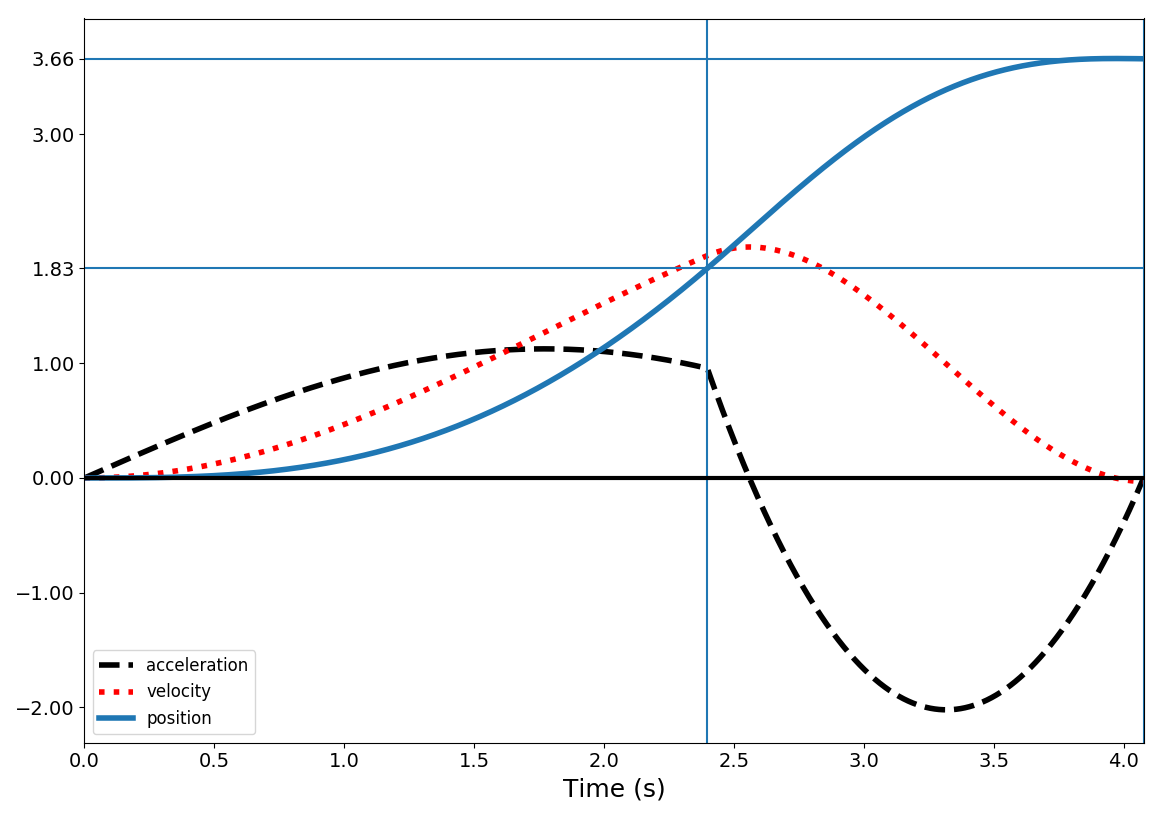
\includegraphics[width=0.8\textwidth]{../img/elevator_acc_dec.png}
    \caption{Acceleration, velocity and position trajectories when elevator decides to stop halfway between floors. Note that floor height is 3.66 meters.}
    \label{fig:motion}
\end{figure}